\documentclass[format=sigconf]{acmart}
\usepackage[english]{babel}
\usepackage{float}
\usepackage[labelfont=bf,textfont=md]{caption}
\usepackage{graphicx}
\usepackage{xcolor}
\usepackage{minted}
\usepackage{hyperref}
\usepackage[all]{hypcap}
\usemintedstyle[glsl]{default}
\usemintedstyle[common-lisp]{default}
\newmintinline[code]{text}{}
\bibliographystyle{unsrt}

\hypersetup{
  colorlinks,
  linkcolor={red!50!black},
  citecolor={blue!50!black},
  urlcolor={blue!80!black}
}

\setcopyright{rightsretained}
\acmDOI{}
\acmISBN{}
\acmConference[ELS'19]{the 12th European Lisp Symposium}{April 1--2 2019}{%
  Genova, Italy}

\setlength{\parskip}{1em}

\begin{document}

\title{Shader Pipeline and Effect Encapsulation using CLOS}

\author{Nicolas Hafner}
\affiliation{%
  \institution{Shirakumo.org}
  \city{Zürich}
  \country{Switzerland}
}
\email{shinmera@tymoon.eu}

\begin{abstract}
  %% FIXME: Abstract
\end{abstract}

\begin{CCSXML}
  %% FIXME: CCS
\end{CCSXML}

\keywords{Common Lisp, OpenGL, GPU, CLOS, Object Orientation}

\maketitle

\newpage

\def\abovecaptionskip{1pt}
\def\listingautorefname{listing}
\def\figureautorefname{figure}

\section{Introduction}\label{introduction}
Modern graphics systems such as OpenGL Core and DirectX offer a lot of customisation to the programmer. Particularly, in order to render an image, they allow the programmer to supply code fragments (shaders) that are run directly on the GPU. These code fragments fill in steps of a fixed rendering pipeline that is executed on the GPU in order to transform vertex data into the pixels of an image. The pipeline for OpenGL is illustrated in \autoref{fig:openglpipeline}.

\begin{figure}[h]
  \begin{center}
    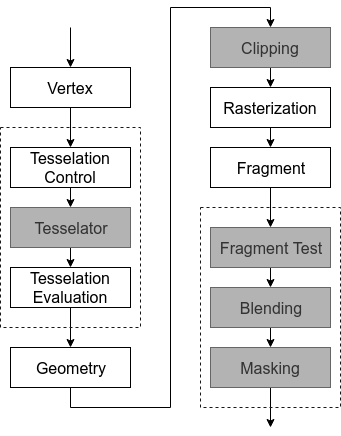
\includegraphics[width=0.3\textwidth]{opengl-pipeline.png}
  \end{center}
  \caption{The stages of the OpenGL rendering pipeline. White boxes represent stages that can be customised with shader code.}
  \label{fig:openglpipeline}
\end{figure}

For consistency, we refer to a step within the hardware rendering pipeline as a ``stage'', an invocation of the hardware pipeline as a ``pass'', and all invocations of the hardware pipeline to produce an image as a ``frame''.

Each of the customisable stages only accepts a single shader for each pass, making it difficult to separate, encapsulate, and ultimately combine behaviour. Furthermore, the steps required in order to change the shaders and shader inputs can be non-trivial and expensive to execute.

The complexity of managing the graphics state and the order of rendering can be massively complicated for modern requirements. Rendering a frame often requires a multitude of passes, each with their own parameters and shared data. The rendering of each object within a pass can also differ, leading to even more state that needs to be correctly managed.

This results in a difficult challenge for modularity. We attempt to solve this challenge through several systems:

\begin{itemize}
\item A protocol for communicating information between a pass and the objects rendered within.
\item A protocol to connect the inputs, outputs, and parameters of different passes.
\item An algorithm to automatically allocate shared textures.
\end{itemize}

\section{Related Work}\label{relatedwork}
Courreges\cite{gtav} presents an in-depth analysis of the rendering procedure employed by the modern, high-production game GTA V. It illustrates the many passes to produce a final image, as well as their data dependencies.

Harada et al.'s work on Forward+\cite{forward+}\cite{forward+talk} also clearly illustrates the need for systems that support multi-pass rendering pipelines with complex data interaction schemes.

Gyrling\cite{fibers} presents an overview of the techniques used to perform parallel rendering in Naughty Dog's commercial engine. Individual stages within a pass, render passes of a frame, and multiple frame renderings are divided up into many small jobs that can run in parallel and are synchronised using counters on a shared structure.

The case study of the Unity game engine by Messaoudi et al\cite{unity} shows the availability of a set of fixed rendering pipelines that can be customised in a very limited extent with custom shaders. However, these shaders must fit into Unity's existing lighting and overall rendering model. While Unity does allow building a custom pipeline via their Scriptable Rendering Pipeline\cite{unitycustom}, they do not seem to offer any specific encapsulation or modularity features.

The work by He et al.\cite{components} introduces a framework for general encapsulation of shaders and their parameters into structures that minimise the overhead of changing GPU state while retaining the ability to dynamically compose shader parts. They do however not create a distinction between properties for the rendering of an object, and those for the rendering of an overall pass.

Foley et al.'s work on Spark\cite{spark} presents a high-level graph-based system for defining reusable and composable shader components. Their system shows a much more distanced view of the underlying graphics hardware than we attempt. Similar to He's work, they do not present a separation between object logic and pass logic.

In our previous work\cite{glsloop} we introduce a system to tie shader code to classes and compose behaviour through inheritance. We make use of this system and extend it to allow further control over rendering behaviour in individual passes.

\section{Overview}\label{overview}

\section{Passes}\label{passes}

\section{Pipelines}\label{pipelines}

\section{Allocation}\label{allocation}

\section{Conclusion}\label{conclusion}


\section{Further Work}\label{furtherwork}


\section{Acknowledgements}\label{acknowledgements}


\section{Implementation}\label{implementation}
An implementation of the proposed system can be found at
\\\href{https://github.com/Shirakumo/trial/blob/f34a79f0a6df21d1ed9259e85fbb3c7eed39352b/shader-pass.lisp}{https://github.com/Shirakumo/trial/blob/\\f34a79f0a6df21d1ed9259e85fbb3c7eed39352b/shader-pass.lisp}
\\\href{https://github.com/Shirakumo/trial/blob/f34a79f0a6df21d1ed9259e85fbb3c7eed39352b/pipeline.lisp}{https://github.com/Shirakumo/trial/blob/\\f34a79f0a6df21d1ed9259e85fbb3c7eed39352b/pipeline.lisp}
\\\url{https://github.com/Shinmera/flow} \\

A more in-depth discussion of the system can be found at
\\\url{https://reader.tymoon.eu/article/363}
\\\url{https://reader.tymoon.eu/article/364}

\bibliography{paper}
\end{document}

%%% Local Variables:
%%% mode: latex
%%% TeX-command-extra-options: "-shell-escape"
%%% TeX-master: t
%%% TeX-engine: luatex
%%% End:
